\documentclass[a4paper]{article}
\usepackage{pdfpages, pgffor}
\setlength{\fboxrule}{0.3mm}

\begin{document}
\newwrite\myoutput
\immediate\openout\myoutput=\jobname.options
\immediate\write\myoutput{\unexpanded{\documentclass[10pt, handout, aspectratio=169]{beamer}}} %43 for 4x3, 169 for 16x9, 1610 for 16x10
\immediate\closeout\myoutput
\foreach \n in {1,...,8}{
    \IfFileExists{week\n/week\n.tex}{
        \immediate\write18{texify.exe --pdf  --clean week\n/week\n.tex}
        \includepdf[pages=-,nup=2x2,delta=5pt 30pt,landscape=true,frame=true,column=false,noautoscale=false]{week\n.pdf}
    }
}
\end{document}

\usetheme{Frankfurt}
\usecolortheme{crane}

\usepackage{exscale,latexsym,microtype,amsmath,amssymb,amsfonts,graphicx,natbib,times,booktabs,xstring}

\newcommand{\E}{\ensuremath{{\mathbb E}}} % expected value
\newcommand{\R}{\ensuremath{{\mathbb R}}}
\newcommand{\Var}{\ensuremath{{\mathbb V}}} % variance
\newcommand{\frameit}[2]{\begin{frame}\frametitle{#1}\begin{itemize}#2\end{itemize}\end{frame}}
\def\func#1{\mathop{\rm #1}}
\def\er#1{\emph{\color{red}#1}}
\def\newblock{\hskip .11em plus .33em minus .07em}
\def\limfunc#1{\mathop{\rm #1}}%
\setbeamertemplate{blocks}[rounded][shadow=true]
\date{}

\titlegraphic{
\includegraphics[height =0.4in]{../HSLU_Logo_EN_Schwarz_rgb}}
\title{Module 9.3: Time Series Analysis with Python\\Fall Term\space\number\year}
\def\theweek{\StrRight{\jobname}{1}}
\author[Week \theweek]{\textbf{Week \theweek}:}
\AtBeginSection{
\frame{
\frametitle{Outline}
\tableofcontents[currentsection]
}}


\institute{{\Large Returns; Autocorrelation; Stationarity}}
\begin{document}
\frame{\titlepage}
\begin{frame}%
\frametitle{Outline in Weeks}
\begin{enumerate}
\item Introduction; Descriptive Modeling
\item Returns; Autocorrelation; Stationarity
\item ARMA Models
\item Unit Roots; ARIMA Models
\item Volatility Modeling
\item Value at Risk
\item Cointegration
%\item Panel Data
\end{enumerate}
\end{frame}% 

\section{Asset Returns}\subsection*{bla}
\begin{frame}
\frametitle{Asset Returns}
\begin{itemize}
\item We consider two definitions of returns:
\begin{enumerate}
 \item \er{Simple} return between dates $t-1$ and $t$ [or: in period $t$]
\[
 R_{t} = \frac{P_{t} - P_{t-1}}{P_{t-1}},
\]
where $P_{t}$ is the asset price at time $t$.

\item Continuously compounded return or \er{log return}
\[
 r_{t} = \log \left ( \frac{P_{t}}{P_{t-1}}  \right ) = \log(1+R_{t}).
\]
\end{enumerate}

\item They are typically very close for daily returns, as
\[
 r_{t} = \log(1+R_{t}) \approx R_{t},
\]
when $R_{t} \approx 0$.
\end{itemize}
\end{frame}

\begin{frame}%
%EndExpansion
\begin{itemize}
\item Log returns and `simple' returns often are very close, as
\[
 r_{t} = \ln(1+R_{t}) \approx R_{t}\mbox{ when } R_{t} \approx 0.
\]
\item Simple returns are bounded below by -1 (100\% loss). Log returns live on $(-\infty, \infty)$. Easier to model (e.g., normal distribution).

\end{itemize}

\begin{block}{Simple vs.\ Log Returns}
\begin{center}
\begin{tabular}{cc}
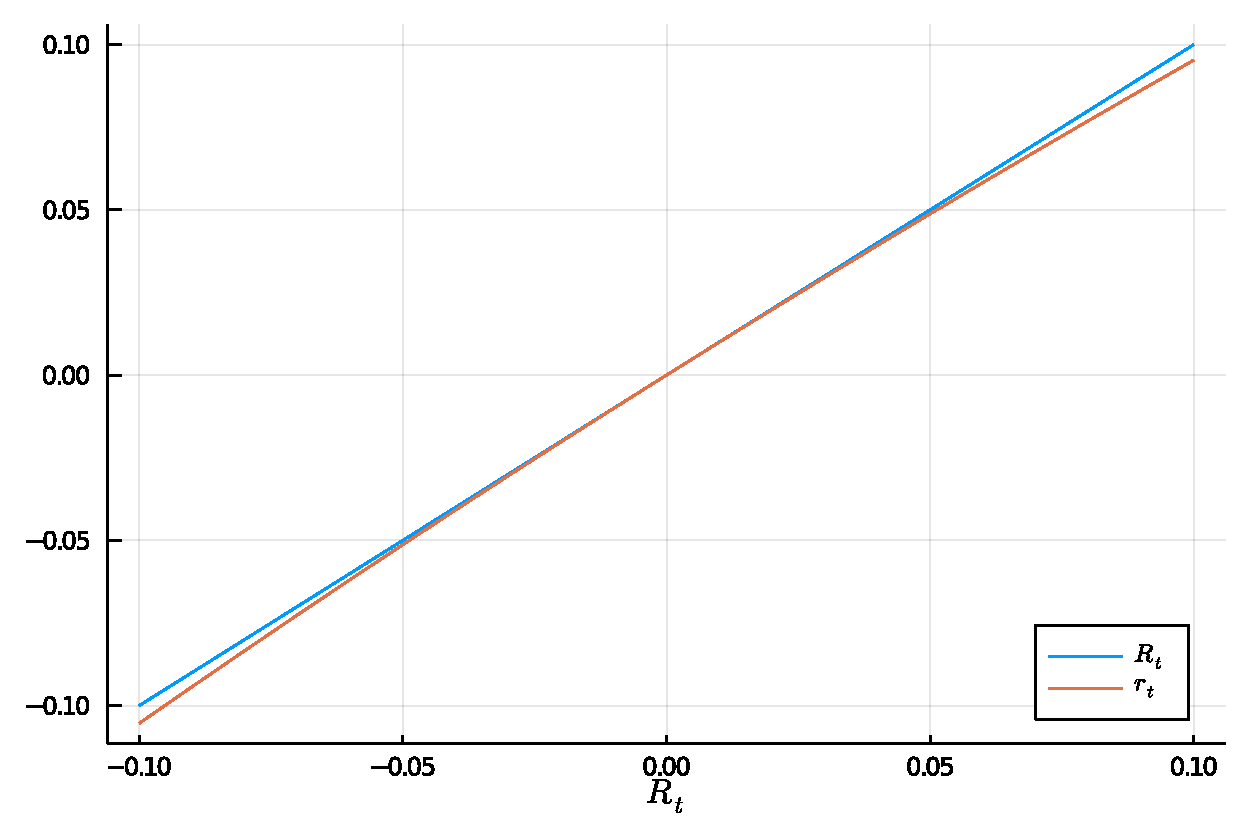
\includegraphics[width=0.35\textwidth]{returns1}&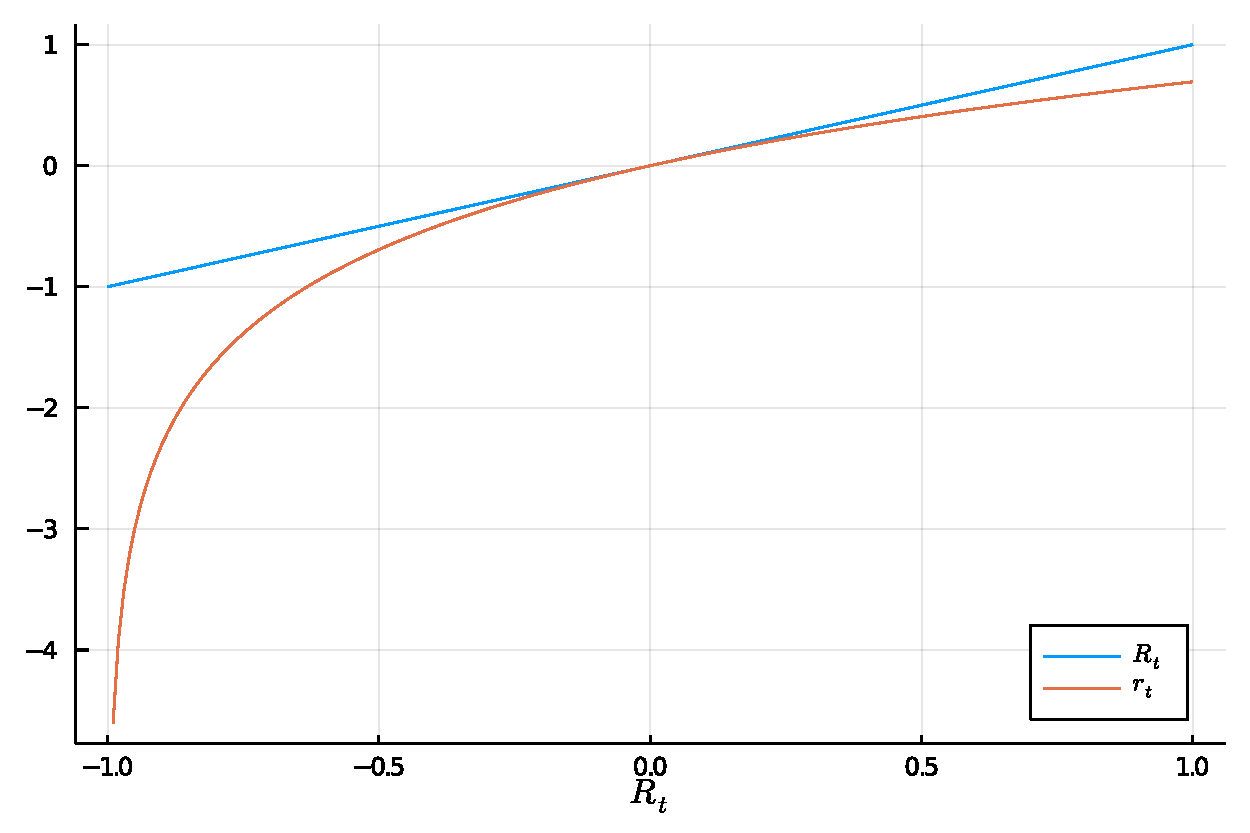
\includegraphics[width=0.35\textwidth]{returns2}
\end{tabular}
\end{center}
\end{block}

%TCIMACRO{\TeXButton{EndFrame}{\end{frame}}}%
%BeginExpansion
\end{frame}%
%EndExpansion
\frameit{Log returns: Intuition}{
\item If a one-period interest rate of $r$ is compounded $n$ times, then
\[
P_t=(1+r/n)^{n}P_{t-1}.
\]
\item  As $n \rightarrow \infty$,
$(1+r/n)^{n} \rightarrow e^{r}$, so
\[
P_t=e^rP_{t-1}\Leftrightarrow r=\log ( P_t/P_{t-1})=\ln  P_t-\log P_{t-1}.
\]

}
\begin{frame}
\frametitle{Portfolio Returns}

\begin{itemize}
\item  Advantage of continuously compounded returns: \er{multi-period return}
is sum of single-period returns.% $r_{t}(k)=r_{t}+\ldots+r_{t-l+1}$, with $r_{t}(k)\equiv \ln(P_{t}/P_{t-k})$.
\item Advantage of simple returns: \er{portfolio return} is weighted sum of
asset returns.
\item Proof: If an investor buys $n_{i}$ shares in stock $i$, then the value of the
portfolio at time $t-1$ is $V_{t-1}=\sum_{i=1}^{n}n_{i}P_{i,t-1}$.

\item Ignoring dividends, the payoff is $V_{t}=\sum_{i=1}^{n}n_{i}P_{i,t}$, so the return
on the portfolio is%
\begin{align*}
R_{p,t}=\frac{V_{t}-V_{t-1}}{V_{t-1}} &=\frac{\sum_{i=1}^{n}n_{i}(P_{i,t}-P_{i,t-1})}{V_{t-1}} \\
&=\sum_{i=1}^{n}\underset{w_{i}}{\underbrace{\frac{n_{i}P_{i,t-1}}{%
V_{t-1}}}\ }\underset{R_{i,t}}{\underbrace{\frac{(P_{i,t}-P_{i,t-1})}{P_{i,t-1}}}}
=\sum_{i=1}^{n}w_{i}R_{i,t}.
\end{align*}


\end{itemize}
\end{frame}
\begin{frame}%
\frametitle{Stylized Facts of Asset Returns}

\begin{itemize}
\item Prices display (time-varying) \emph{\color{red}trend}, and variation
proportional to price level (motivation for taking logs).

\item Returns have constant mean close to zero, and very little
autocorrelation.

\item Returns display \emph{\color{red}volatility clustering}: alternating periods of
high and low variability.

\item Returns have non-Gaussian distribution, \emph{\color{red}fat tails} (excess
kurtosis).

\item Interest rates display long swings, very slow \emph{\color{red}mean-reversion}.

\item Interest rate changes have similar characteristics as returns.
\end{itemize}
\end{frame}%
\begin{frame}%
\begin{block}{\emph{Example}: S\&P 500 index values and returns, 10/29/2012--10/27/2022}
\begin{center}
\begin{tabular}{rr}
\includegraphics[height=0.3\textheight]{sp500}&\includegraphics[height=0.3\textheight]{sp500_log_price}\\
\includegraphics[height=0.3\textheight]{sp500_return}&\includegraphics[height=0.3\textheight]{sp500_hist}
\end{tabular}
\end{center}
\end{block}
\end{frame}%
%\begin{frame}%
%\begin{block}{\emph{Example}: 3 Month T-Bill rate, 10/29/2012--10/26/2022}
%\begin{center}
%\begin{tabular}{rr}
%\includegraphics[height=0.3\textheight]{dtb3}&\includegraphics[height=0.3\textheight]{diffdtb3}\\
%&\includegraphics[height=0.3\textheight]{histdtb3}
%\end{tabular}
%\end{center}
%\end{block}
%\end{frame}
\begin{frame}
\frametitle{Testing Normality}
\begin{itemize}
\item Normality can be tested
by examining the \emph{\color{red} skewness} and \emph{\color{red}kurtosis}.


\item Skewness $\text{SK}=m_{3}/\sqrt{m_{2}^{3}} \text{ and kurtosis K}=m_{4}/m_{2}^{2}$,
where $m_{j}$ is the $j$-th centralized moment\footnote{I.e., the second centralized moment $m^2$ is just the variance, otherwise known as $\sigma^2$.}
$m_{j}=\E[(r_{t}-\E[r_{t}])^{j}]$.

\item A normal distribution has SK=0 and K=3.

\item\emph{\color{red}Jarque-Bera normality test}:
\[ \text{JB} = \frac{T}{6}\widehat{\text{SK}}^{2} +
   \frac{T}{24}(\widehat{\text{K}}-3)^{2}, \]
where the skewness and kurtosis of $r_{t}$ can be estimated as
\[
  \widehat{\text{SK}} =
  \hat{m}_{3} / \sqrt{\hat{m}_{2}^{3}}, \quad \text{and} \quad
  \widehat{\text{K}} = \hat{m}_{4} / \hat{m}_{2}^{2}, \quad \text{with } \hat{m}_{j} = \frac{1}{T} \sum_{t=1}^{T}
(r_{t}-\overline{r})^{\;j}.
 \]
\item Under the null hypothesis of normality:  $\mathrm{JB}\;{\overset{d}{\longrightarrow }}\;
\chi_{2}^{2}$.
\end{itemize}
\end{frame}
\section{Stochastic Processes}\subsection*{bla}
\frameit{Stochastic Processes}{
\item Time series analysis is concerned with modelling,
estimating, analyzing and forecasting returns and other financial and economic variables.

\item A \emph{\color{red}time series} $\{y_t,t=1,2,\ldots ,T\}$ is a collection of
subsequent observations on a particular variable. We view such a time series
as a \emph{\color{red}realization} of a \emph{\color{red}discrete-time
stochastic process} $\{Y_t,t=1,2,\ldots \}$, which is a collection of
(dependent) random variables.
\item The goal is to determine which process $\{Y_t\}$ generated the data.
\item  The distinction between $\{Y_t\}$ (the
process) and $\{y_t\}$ (the realization) will usually not be emphasized.
\item
We
will not consider continuous-time stochastic processes here (e.g.\ Brownian
motion).

}
\begin{frame}
\frametitle{White Noise}
\begin{itemize}
\item  An important example of a stationary process is the \er{white noise} process, which has zero mean\footnote{Brooks allows a white noise process to have a non-zero mean. Usually such a
process is called an \emph{\color{red}uncorrelated} process.} and zero autocovariances.
\begin{eqnarray*}
\E[U_{t}] &=&0, \\
\mathrm{var}(U_{t}) &=&\E\left[U_{t}^{2}\right]=\sigma ^{2}, \\
\mathrm{cov}(U_{t},U_{t-k}) &=&\E[U_{t}U_{t-k}]=0,\qquad k=1,2,\ldots
\end{eqnarray*}%
\item The notation $U_t$ emphasizes the similarity to regression errors.
\item White noise is \er{unpredictable}.
\item It is the building block for other processes (which may be predictable).
\end{itemize}
\end{frame}
\section[The EMH]{The Efficient Market Hypothesis}\subsection*{bla}
\frameit{Excursus: The Efficient Market Hypothesis}{
\item The \er{weak form EMH}\footnote{Fama (1970). Efficient Capital Markets: A Review of Theory and Empirical Work. \emph{Journal of Finance}, 25(2), pp.\ 383--417.} posits that past prices and returns cannot predict future returns.
\item This implies that no fund manager can consistently outperform the market, at least based on historical prices alone.
\item If weak form EMH holds, then returns should be \er{uncorrelated}. Since the mean return is small for daily data, they should therefore resemble wight noise.
\item An important application of time series analysis ist testing whether the EMH holds.
\item The most basic way to do this is to test whether the returns have been generated by a white noise process.
}
\section[The ACF]{The Autocorrelation Function}
\begin{frame}
\frametitle{Autocorrelation Function}
\begin{itemize}
\item Recall that if a process $\{Y_t\}$ is white noise, then it is uncorrelated at all lags (i.e., $Y_t$ should be uncorrelated with $Y_{t-1}$, with $Y_{t-2}$, etc.)
\item Formally, its \emph{\color{red}autocorrelation function (ACF)} $\tau_s$ is zero for all $s$, where the ACF is defined from the \emph{\color{red}autocovariances} $\gamma_s$, as
\begin{equation*}
\tau _{s }=\func{Corr}(Y_{t},Y_{t-s })=\frac{\func{Cov}%
(Y_{t},Y_{t-s })}{\func{Var}(Y_{t})}=\frac{\gamma _{s }}{\gamma _{0}}%
,\qquad s =1,2,\ldots
\end{equation*}
\end{itemize}
\end{frame}
\frameit{PSA: Population vs.\ Sample Quantities}{
\item It is important to note that the ACF is a property of a \er{process}, not of a \er{sample} (i.e., the observed time series). This makes them \er{population quantities} or \er{parameters}.
\item The statement on the previous slide says that the random variables $\{Y_1, Y_2, \ldots\}$ generated by a white noise process are uncorrelated.
\item Population quantities are \er{unobserved}. The best we can hope for is to \er{estimate} them from a sample (a time series).
}
\frameit{PSA: Population vs.\ Sample Quantities}{
\item To use the normal distribution as an analogy: it has two parameters, $\mu$ and $\sigma^2$. These are \er{parameters} and thus \er{unobserved}.
\item In a simulation exercise, I can \er{pretend} to know what $\mu$ and $\sigma^2$ are.
\item E.g., I can set $\mu=0$ and $\sigma^2=4$, simulate 1000 random numbers $y_t$, and give them to you.
\item Unlike me, you won't know what $\mu$ and $\sigma^2$ are. At best, you can \er{estimate} them, based on the \er{sample mean and variance}
\[
\bar{y}\equiv\frac{1}{N}\sum_{i=1}^N y_i\quad \text{and}\quad s^2_y\equiv\frac{1}{N}\sum_{i=1}^N (y_i-\bar{y})^2.
\]
\item If the sample is large enough, then these will be \er{close} to $\mu=\E[Y]$ and $\sigma^2=\func{Var}(Y)$ by the law of large numbers (\er{LLN}).
}
\begin{frame}
\frametitle{The Correlogram}
\begin{itemize}
\item Applying the analogy to the ACF, the
\emph{\color{red}Sample ACF} or \emph{\color{red}correlogram} is defined as
\begin{equation*}
\hat{\tau}_{s }=\frac{\hat{\gamma}_{s }}{\hat{\gamma}_{0}}=\frac{%
\sum_{t=s +1}^{T}(y_{t}-\bar{y})(y_{t-s }-\bar{y})}{%
\sum_{t=1}^{T}(y_{t}-\bar{y})^{2}},\qquad \bar{y}=\frac{1}{T}%
\sum_{t=1}^{T}y_{t}.
\end{equation*}
\item The correlogram is a \er{sample quantity}, i.e., I can compute it from a given time series.
\item If I want to test if the time series is white noise, I can compare my SACF to the ACF of a white noise process.
\item If the two are significantly different, then I can reject the null that the time series was generated by a white noise process.
\item See exercises and the spreadsheet \texttt{simulations.xlsx}.
\end{itemize}
\end{frame}
\begin{frame}
\frametitle{Testing if an Autocorrelation is Zero}
\begin{itemize}
\item One can show that under the null that the data were generated by a white noise process, the sample autocorrelations are asymptotically\footnote{Formally: under $H_{0}:\tau _{s }=0,s \geq 1$, $\sqrt{T}\hat{\tau}_s \overset{d}{\longrightarrow }N(0,1)$.} normally distributed with
zero mean and variance $1/T$.
\item This implies that a sample autocorrelation is significantly different from
zero if its absolute value is larger than $1.96 / \sqrt{T}$.

\item We can also test whether the first $m$ autocorrelations are zero jointly: under $H_{0}:\tau _{s }=0,s \geq 1$, the \emph{\color{red}Ljung-Box}  $Q$-statistic%
\begin{equation*}
Q(m)=T(T+2)\sum_{s =1}^{m}\frac{\hat{\tau}_{s }^{2}}{T-s }\quad
{\overset{d}{\longrightarrow }}\quad \chi ^{2}(m).
\end{equation*}%
\end{itemize}
\end{frame}%
%\begin{frame}
%\begin{block}{\emph{Example}: Daily Dow Jones index returns, Jan 1, 1990 - Dec 31, 2005}
%\centerline{\includegraphics[height=2in]{acfs.png}}
%\end{block}
%\end{frame}
\begin{frame}
\begin{block}{Example: Correlogram of S\&P500 returns}
\begin{center}
%\includegraphics[width=0.3\textwidth]{correlogram}
\includegraphics[width=0.5\textwidth]{sp500_acf}
\end{center}

\end{block}
\begin{itemize}
\item The shaded blue area represent the critical value of $1.96 / \sqrt{T}=0.039$, so, e.g., the autocorrelations at lags 1 (-0.145) and 2 (0.092), are significant, while the one at 3 (0.0116) is not.
\end{itemize}
\end{frame}

\begin{frame}
	\begin{block}{Example: $Q$-stats for S\&P500 returns}
		\begin{center}
			%\includegraphics[width=0.3\textwidth]{correlogram}
			\includegraphics[width=0.2\textwidth]{q-stats}			
		\end{center}
		{\footnotesize E.g., $Q(5)=88.86$ can be used to test the null that the first 5 autocorrelations are jointly zero. The critical value is 11.07, so the test rejects.}
	\end{block}
	\begin{itemize}
		\item The $Q$ statistics confirm the presence of autocorrelation ($p$-values less than 5\%).
		\item Conclusion: some autocorrelation, and hence predictability, in the returns; returns are not white noise. Unclear if predictability is sufficient to exploit with a trading strategy.
	\end{itemize}
\end{frame}

\section{The Random Walk}\subsection*{bla}

\frameit{From Returns to Asset Prices}{
\item We have seen that the EMH suggests that white noise is a reasonable model for stock returns:
\[
r_t=U_t, \quad\text{where } U_t \text{ is white noise (not necessarily normal)}.
\]
\item Recall the definition of log returns:
\[
r_t=\log P_t-\log P_{t-1}.
\]
\item Putting the two together implies that
\begin{align*}
\log P_t-\log P_{t-1}&=U_t\Leftrightarrow\\
\log P_t&=\log P_{t-1}+U_t.
\end{align*}
\item This characterizes the log asset price as a \er{random walk}.
}
\begin{frame}
\begin{block}{Definition}
A \er{random walk} is the stochastic process
\[
Y_t=Y_{t-1}+U_t,
\]
where $U_t$ is white noise and $Y_0$ is some fixed starting value.
\end{block}
\end{frame}
\frameit{Properties of the Random Walk}{
\item The random walk behaves very differently from white noise.
\item A quick calculation shows that
\[
Y_t=Y_0+U_1+U_2+\cdots+U_t=Y_0+\sum_{s=1}^t U_s.
\]
\item From this, it is immediate (see exercises) that
\begin{align*}
\E(Y_t)&=Y_0\quad\mbox{and} \\
\mathrm{var}(Y_t)&=\sigma ^2t.
\end{align*}
\item One can also show that
\[\mathrm{corr}(Y_t,Y_{t-k})=\sqrt{(t-k)/t}.\]

}
\frameit{Properties of the Random Walk}{
\item In words:
\begin{itemize}
\item The effect of a ``shock'' $U_t$ is permanent; $U_t$ is in all future values $Y_s, s\geq t$, whereas for a white noise process, $U_t$ only affects $Y_t$.
\item The variance increases over time, because we add up more and more of the $U_t$, all of which are random.
\item The correlogram decreases slowly, approximately linearly (see also \texttt{simulation.xlsx}).
\end{itemize}
\item We say that a random walk is not \er{mean reverting}; one can show that it will (eventually) hit each and every level $L$, and its excursions can take arbitrarily long.



}
\section[I(0) and I(1) Processes]{Stationary and Integrated Processes}\subsection*{}
\frameit{Stationary Processes}{
\item Earlier, we rejected the null that the returns on the S\&P500 are white noise (although they are close).
\item This also implies that the log stock prices are not (exactly) random walks.
\item This means that we need to generalize these concepts to allow for other types of stochastic process.
\item Specifically, instead of pure white noise, we will consider \er{stationary processes}.
\item Similarly, we generalize the concept of a random walk to \er{integrated processes}.
\item Specific instances of these processes (ARMA and ARIMA models, respectively) will be considered in Weeks 3 and 4.
}

\begin{frame}\frametitle{Stationarity}%
\begin{block}{Definition}
A process $\{y_{t}\}$ is called \emph{\color{red} weakly stationary} (or second-order, covariance stationary) if
the first two moments are time-invariant:%
\begin{equation*}
\E[Y_{t}]=\mu ,\quad \func{var}(Y_{t})=\gamma_0=\sigma^2, \quad \func{cov}(Y_{t},Y_{t-s })=\gamma _{s },\quad
 t\in \{0,\ldots, T\},s \geq 1.
\end{equation*}%
\end{block}
\begin{itemize}
\item This means that the mean, variance, and autocovariances (or autocorrelations) do not change over time; i.e., the autocovariance $\gamma_s$ depends only on the lag $s$, not on $t$.
\item Intuitively, there should not be a significant difference if I calculate the mean, variance, and ACF from the first or second half of the sample.
\item White noise is one example of a \er{stationary} process.
\item As we saw, the random walk is not stationary; its variance changes over time.
\end{itemize}
\end{frame}%
\frameit{Integrated Processes}{
\item Recall that if returns are white noise, then log prices follow a random walk:
\[
\log P_t  = \log P_{t-1}+ U_t
\]
\item Alternatively, if log prices follow a random walk, then returns are white noise:
\[
r_t=\log P_t - \log P_{t-1} = U_t
\]
\item We write $\Delta \log P_t$ for $\log P_t - \log P_{t-1}$.
\item So a process $Y_t$ is a random walk if $\Delta Y_t$ is white noise.
}
\begin{frame}
\frametitle{Integrated Processes}
\begin{itemize}
\item We saw above that for the S\&P500, we did not get white noise after differencing, but some other stationary process.
\item Such processes are called \er{integrated}.
\end{itemize}
\begin{block}{Definition}
A process $Y_t$ is called \emph{\color{red}integrated} of order 1, or \er{I(1)}, if it
is non-stationary itself, but $\Delta Y_t = Y_t - Y_{t-1}$ is stationary.
\end{block}
\begin{itemize}
\item The random walk is the simplest example of an I(1) process.
\item A stationary process is also called \er{I(0)}.
\item An I(2) process would need to be differenced twice to be stationary, but this is rarely necessary in practice.
\end{itemize}
\end{frame}
\begin{frame}
\frametitle{Properties of Integrated Processes}
\begin{itemize}
\item  Integrated processes have correlograms that stay close to one, which \er{die out very slowly}.
\item An informal way to check whether the stationarity assumption is
reasonable is by inspecting the graph and the correlogram of the series. If
the graph displays a tendency to revert to a constant mean, with a
more or less constant variance, and the correlogram converges to zero
\er{exponentially fast}, then stationarity may be assumed. A formal test will be introduced later.
\item Besides prices, many financial and economic time series (e.g., GDP) do not seem to be stationary,
because they display a trending mean, and a variance that increases with the
level of the process. The latter phenomenon is usually dealt with by a
log-transformation, but then quite often the series is still not stationary.
\end{itemize}
\end{frame}
\begin{frame}
\begin{block}{Example: ACF of S\&P500 returns and log prices}
\begin{centering}
\begin{tabular}{cc}
\includegraphics[width=.45\textwidth]{sp500_acf}&
\includegraphics[width=.45\textwidth]{sp500_acf_levels}
\end{tabular}
\end{centering}
\end{block}
\end{frame}
\begin{frame}
\frametitle{Note: Partial Autocorrelation Function}
\begin{itemize}
\item A concept related to the ACF is the (sample) \emph{\color{red}partial
autocorrelation function} ((S)PACF) $\hat{\tau}_{kk},k=1,2,\ldots $
, where $\hat{\tau}_{kk}$ is the OLS\ estimator of $%
\tau _{kk}$ in the regression
\begin{equation*}
y_t=\alpha +\tau _{k1}y_{t-1}+\ldots +\tau _{kk}y_{t-k}+e_t.
\end{equation*}
\emph{\color{red}Note}: this is not the model for $y_t$, just a regression
to estimate $\tau _{kk}$!
\item The PACF measures the correlation between $y_t$ and $y_{t-k}$, \er{controlling} for the effect of the intermediate lag. I.e., $\tau _{kk}$ only
measures the \er{direct} effect of $y_{t-k}$ on $y_t$.
\item For a random walk, it drops to zero after the first lag, because only $y_{t-1}$ has a direct effect.
\item For a stationary process, the ACF and PACF
converge to zero at a geometric (exponential) rate as $k$ increases.
\item
If the sample ACF and PACF of a time series
do not seem to converge at all, or too slowly (linearly), then this is an
indication of nonstationarity.
\end{itemize}
\end{frame}
\begin{frame}
	\begin{block}{Example: PACF of S\&P500 returns and log prices}
		\begin{centering}
			\begin{tabular}{cc}
				\includegraphics[width=.45\textwidth]{sp500_pacf}&
				\includegraphics[width=.45\textwidth]{sp500_pacf_levels}
			\end{tabular}
		\end{centering}
	\end{block}
\end{frame}
\begin{frame}{More Properties of Integrated Series}
\begin{itemize}

\item \er{No mean-reversion}. Like the random walk, I(1) processes do not revert to a mean.
\item \er{Persistence of shocks}. Also,
the effect of past shocks $u_{t-i}$ does not die out, whereas for stationary
series the effect will decay exponentially. Important for
economic policy.

\item \er{Increasing forecast intervals}. For I(0)
time series, the long-run $95\%$ forecast interval converges to the
unconditional mean $\pm$ twice the unconditional standard
deviation. For an I(1) process the forecast variance does
not converge, so forecasts intervals keep increasing.

\item \er{Spurious regressions}. When regressing two
integrated time series onto each other, the $R^{2}$ and $t$-statistic may become very
large even if they are totally independent. This is avoided if we regress $%
\Delta y_{t}$ on $\Delta x_{t}$.

\item \er{Asymptotic properties of estimators and tests}. In regressions with I(1) variables, the usual statistical theory breaks down (asymptotic normality of estimators, $t$-tests, etc).
\end{itemize}
\end{frame}





\section{Epilogue}\subsection*{bla}
\frame{
\frametitle{Learning Goals}
Students
\begin{itemize}
\item know the definitions of simple and log returns,
\item know the definition of white noise,
\item understand the ACF and PACF and their sample analogs,
\item are able to use the correlogram and $Q$-statistics to test if a series was generated by a white noise process, and
\item are able to distinguish stationary and integrated processes.
\end{itemize}
}
\frameit{Homework}{
\item Exercise 2
\item Questions 9b and 12b from Chapter 6 of Brooks (2019)
}
\end{document}
